\documentclass[english]{tktltiki}
\usepackage[pdftex]{graphicx}
\usepackage{subfigure}
\usepackage{url}
\usepackage{amsmath}
\usepackage{algorithm}
\usepackage[noend]{algpseudocode}

\newcommand\floor[1]{\lfloor#1\rfloor}
\newcommand\ceil[1]{\lceil#1\rceil}
\def\doubleunderline#1{\underline{\underline{#1}}}

\begin{document}
\onehalfspacing

\title{Location Awareness - Week 1}

\author{P�ter Ivanics}
\date{\today}

\maketitle

\numberofpagesinformation{\numberofpages\ pages}

\mytableofcontents
 
\section{Location-based Services} 
	In the following subchapters, four Location Based Services (hereinafter LBSs) are introduced briefly. The first three - Commuter, Sports Tracker and Frank - are consumer applications. They show some similarities in their business model and targeted audience as they freely available for everyone on today's popular mobile platform (iOS, Android and Windows Phone). However, they differ in their functionality as Commuter supports the usage of public transportation, Sports Tracker encourages the community to do physical exercises, while the Frank is an application that helps students getting around and claim discounts in Finland. The reason for describing these applications is their popularity, different focus and application area. As an active end-user, I have hands-on experience in all of them. In my opinion these applications are great specimen for this assignment.
	
	The last example is a mobile workforce management platform called Reslink. The reason of choosing this platform is its wide applicability, rich data and different focus compared to the other examples. In comparison to the previous examples, Reslink is a business-to-business platform operating in multiple business verticals. As one of the developers of the Reslink platform I believe that it serves as a splendid example of a LBS in the business field of workforce management.
	
	\subsection{Commuter}
		% What is this solution briefly? Who is the targeted audience? 
		Commuter \cite{com16} is a simple, but tremendously useful application for people living all around Finland. The service allows users to look for routes from point A to point B using the public transportation. As soon as the source and destination is known, the application suggests the fastest transits to get to the destination, which can be by using bus, tram, underground, train or walking. Routes can be planned on demand or in advance by defining the desired arrival time. The starting point for the journey is the current location of the user, but it can be defined differently for each journey, if needed. While on the road, the service guides the user where he/she is currently on the map, shows the upcoming stops and reminds the user for transitions between lines. Figure \ref{commuter_planning} shows an example journey from Kumpula to the center of Helsinki on bus number 722 in the application. The application has many other features, such as listing nearby bus stops, bookmarks, favorite lines, route history, reminders, disruptions, service points and so on. The service is available on iOS devices.
		
		\begin{figure}[h] 
			\begin{center}
			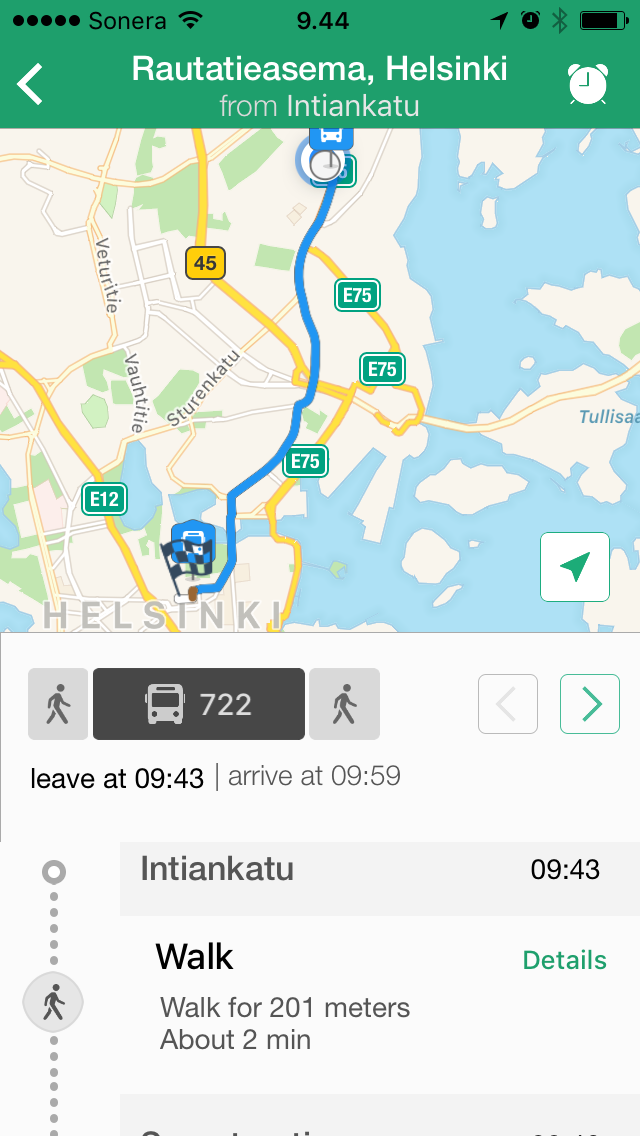
\includegraphics[height=0.6\textwidth]{images/commuter-planning.png}
				\caption{Planning a journey from Kumpula to the Helsinki railway station in Commuter.}
				\label{commuter_planning}
			\end{center}
		\end{figure}
		
		% How this solution uses location awareness? 
		The application relies very much on the location of the user just like any navigation and transportation service. The user's location is visible all the time in the application even if the starting point of a journey differs. Users are continuously shown their surroundings, such as street map, bus stops, stations and service points. While on journey, it is clearly indicated what the upcoming stops are and how long time it takes to reach the desired destination. The transition between lines could never be easier than with this service as is indicates the distance and direction clearly. All in all, this service greatly enhances the location awareness of the user and helps to reach the intermediate and final destinations.
		
		% How does this solution address the challenges? Lack of standards, Positioning, Power consumption, Privacy
		Commuter addresses the challenges as follows. 
	\begin{itemize}
		\item Lack of standards: the service is focused on one mobile platform as it is available only on iOS devices. From the "About" page in the application it is clear that different public APIs are utilized for the accurate data displayed in the application. This means that the timetables of the public transportation and disruptions are loaded from public data sources. These sources are unknown; there is a possibility that they are different format but yet transparent for the user.
		\item Positioning: the positioning works very accurately as an end-user even without internet connection. Seemingly, the position is updated every couple of seconds, which gets a bit more rapid when on journey. This is logical, because users need more updates while using on public transport than when planning their journey.
		\item Power consumption: as an end-user, the application consumes fairly small amount of battery. The service is limited to access data only from a limited number of sensors. For example, it would not benefit from the usage of the camera or microphones and therefore does not use these accessories at all, which saves some battery power.
		\item Privacy: users are not required to enter any log-in credentials nor e-mail addresses in advance of using the applicaiton. This indicates anonymity as an end-user and homogeneity among the user base. If the service provider collects data concerning users, their identity should remain unknown, however their behavior and habits could be interesting to analyze.
	\end{itemize}
	
	\subsection{Frank}
		% What is this solution briefly? Who is the targeted audience?
		Frank \cite{fra16} is an application that helps students to find stores and activities that offer student discounts all around in Finland. Such places can be listed or displayed on the map. The application also offers filtering possibilities based on the offered services, for instance grocery stores, restaurants, hardware stores, entertainment, sport centers ant so on (Figure \ref{frank-places-in-helsinki}). The results in the list representation can be ordered based on the distance from the user's current position. The service also allows students to register their digital student card and use the application to prove their identity. By presenting their student card and the application at the counter, students are able to claim discounts at the listed locations. Last but not least, once students register, they may retrieve seasonal discounts and bonuses. The application is available on iOS and Android platforms.
		
		\begin{figure}[h] 
			\begin{center}
			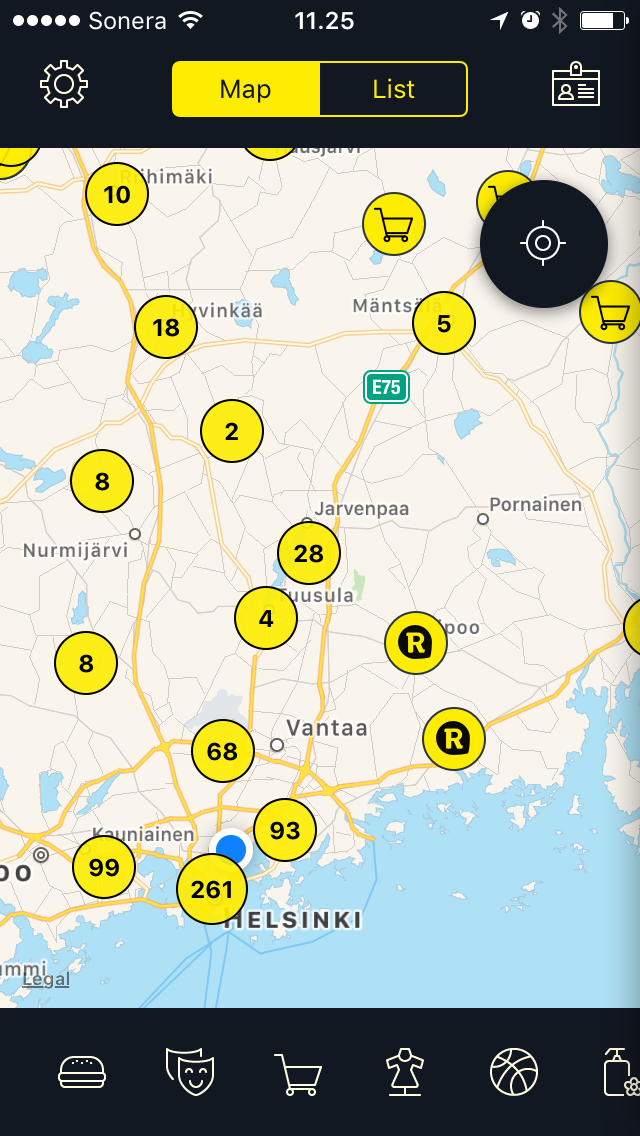
\includegraphics[height=0.6\textwidth]{images/frank-places-in-helsinki.png}
				\caption{A visualization of stores offering student discounts through the Frank application around Helsinki.}
				\label{frank-places-in-helsinki}
			\end{center}
		\end{figure}
		
		% How this solution uses location awareness? 
		This solution uses location awareness by listing and displaying users the points of interest in their neighborhood. The application has the capability to retrieve the location of the user even in offline mode. However, listing the places that offer discounts is only possible while connected to the Internet. Location awareness is enhanced by displaying the results on the map and providing the possibility to order the results based on the distance from the current position.
		
		% How does this solution address the challenges? Lack of standards, Positioning, Power consumption, Privacy
		Frank addresses the typical challenges as follows:
		\begin{itemize}
			\item Lack of standards: as the application supports multiple platforms, the lack of standards was surely overcome. Engineers at Frank must have developed some standard APIs for their platform that allows the communication between components easily. 
			\item Positioning: the application does not require too much of location tracking and positioning. The user's location is retrieved once when the application is started, and most likely polled periodically during its lifecycle. 
			\item Power consumption: the application seems to consume very small amount of battery power as only a few sensors are utilized for its functionality. 
			\item Privacy: privacy comes to question only if students register their digital student cards. Before doing so, they are completely anonymous. By knowing the identity of the users by their social security number, their personality and student status can be validated. Ultimately, it could be even tracked, what kind of places they are interested in, where do they visit and what kind of discounts they are looking for. This kind of information can be essential for stores to maximize sales and marketing potential. 
		\end{itemize}			
	
	\subsection{Sports tracker}
		% What is this solution briefly? Who is the targeted audience? 
		Sports Tracker is a service that connects location awareness with sports and exercises. The idea is that end-users use the location information generated by their mobile devices to track the route on which they were working out. The data is then visualized on the map, calculate exercise statistics and performance indicators, how long the exercise lasted, how many calories were burned and so on. The results may differ depending on which kind of exercise the user performs, for instance cycling, skiing, jogging or walking. For instance, Figure \ref{sports-tracker-midnight-run} shows one of my running workouts. On top of that, the service provides many other features such as integration with social network, sharing workout data, taking and sharing photos, comparison to and competition with other users, notifications about friends' workouts and so on. Each user has a personal profile which can be accessed through a web-based backend platform. The application is available on the three main platforms.
	
		\begin{figure}[h] 
			\begin{center}
			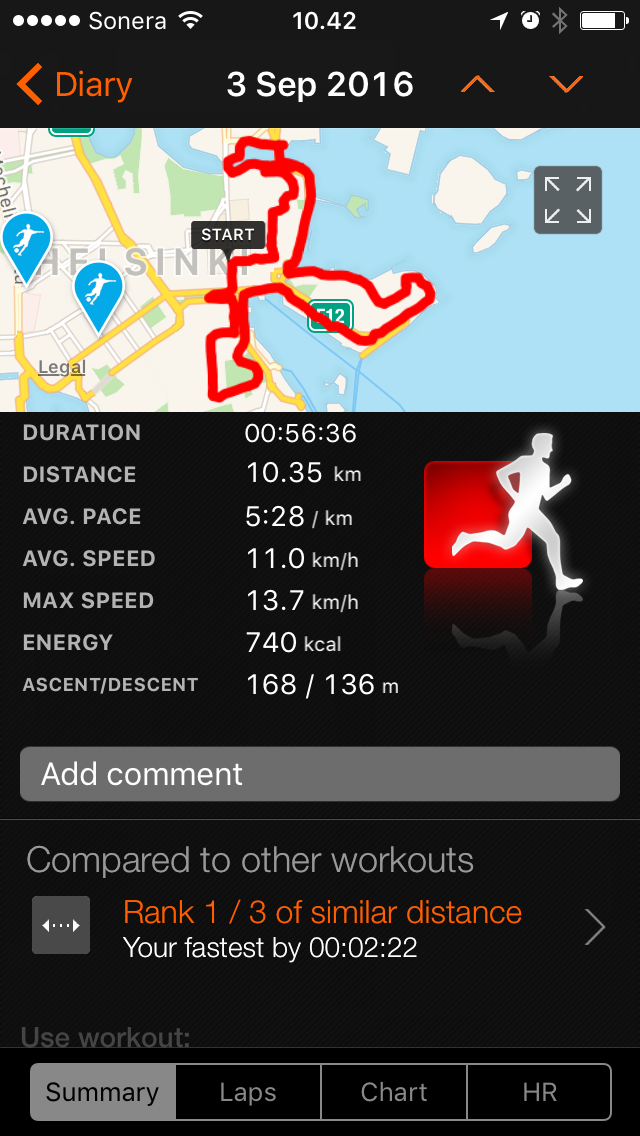
\includegraphics[height=0.6\textwidth]{images/sports-tracker-midnight-run.png}
				\caption{My statistics collected through the Sports Tracker application during the Helsinki Midnight Run.}
				\label{sports-tracker-midnight-run}
			\end{center}
		\end{figure}		
		
		% How this solution uses location awareness? 
		The application relies very much on the location and accelerometer data of the device. This data is utilized for calculating the number of steps, distance traveled and calories burned during the workout. Obviously, the same data is utilized to visualize the workout-route on the map. Naturally, the application works the best for working out outside, but it can be used for training indoors as well. During a workout users can retrieve detailed information concerning their performance and position which can help them to decide how they would like to proceed with their current workout. 
		% How does this solution address the challenges? Lack of standards, Positioning, Power consumption, Privacy
		The challenges in this case are addressed in the following way: 
	\begin{itemize}
		\item Lack of standards: as the application supports three platforms, the Sports Tracker platform has to have well defined APIs. The mobile clients are surely conform to the end-points and submit the data to the database in the defined format. This is an impressive achievement as it is completely transparent for end-users on different platforms.
		\item Positioning: the positioning is more or less accurate. In the past I personally noticed some errors after looking at my workouts. This indicates that the application attempts to save energy on the cost of accurate positioning, which is a wise decision. Nevertheless, the displayed location information is very relevant and accurate after all in most of the cases.
		\item Power consumption: in my experience, the application consumes moderate amount of battery power. This is not a surprise considering that multiple sensors are utilized for data collection. Interestingly, the application is fully operational without stable internet connection, which indicates trust on fewer sensor data as well.
		\item Privacy: as users have their own training profile and form a community, privacy is a relevant question in this case. The application collects huge amount of data concerning the exercises and individuals' health information, which can violate individuals' views on the question of privacy. For this reason, users can decide if they share workout information to the public, their friends or keep it private. On the other hand, this data can be valuable to indicate healthfulness of users, to detect and avoid potential health-related issues.
	\end{itemize}		
		
	\subsection{Reslink}
		% What is this solution briefly? Who is the targeted audience?
		Reslink \cite{res16} is targeting organizations that utilize workforce at various locations. The offering is not limited to an application or LBS, but extends to a complete workforce management platform. Customers of Reslink can design their own business application, which is then installed on the employees' mobile devices in order to allow them performing their job on the field. The platform is flexible enough to serve the needs of different business verticals, such as security guarding, home care, cleaning, technical maintenance, brewery or facility management. In essence, the mobile applications aim to replace paper-based work and collect rich digital data from the field of operations. The data may include both qualitative and quantitative types, such as textual, numerical, location data or photos, audio and video recordings. The service supports mainly Android and iOS platforms but has limited capabilities on Windows Phones as well.
		
		% How this solution uses location awareness? 
		Location awareness is utilized through this service in various ways. Employees can plan their workday and navigate between locations easily as the day goes on. In addition, managers can control and monitor their workforce from the back-office, while employees use a single device to move on the field and to perform their job. Ultimately, it is possible to supervise where the employees are, as well as to get immediate feedback if something unexpected happens on the work-field. As an example, imagine a security guard reporting vandalism in one of the facilities by uploading a video or picture. In such situation, supervisors are notified via e-mail or text messages that allows them to immediately delegate resources to the location where the incident has happened. The solution also offers many additional features like Geo Fencing, GPS position tracking, locationing through NFC tags and barcodes. 
		
		% How does this solution address the challenges? Lack of standards, Positioning, Power consumption, Privacy
		Plenty of challenges arise in such platform. Some of them are, as follows:
		\begin{itemize}
			\item Lack of standards: supporting all three mobile platforms is a major challenge. Despite the fact that communication protocols between the clients and the back-office are standard, the mobile clients face some limitations due to the inconsistency between the mobile operating systems. 
			\item Positioning: depending on the customer cases, accurate positioning may have different level of importance. In some cases, positioning may be challenging due to weak network signal strength. For example, if a technician is working at a customer location in the basement, the device might go completely offline but reporting that the work was done at exaclty this location is crucial. Reslink overcomes this challenge by providing full offline-mode support and storing all transactions in the memory of the device. As soon as the device retrieves stable internet connection, the data is sent to the back-office, which embeds indicators concerning the accuracy of the data. 
			\item Power consumption: depending on the utilized features, Reslink mobile clients may consume lot of battery power. For instance the GPS tracking feature can be configured in a way to poll the location of the device every minute, which drains lots of energy from the power source. For this reason, the employees' and applicaitons' settings are fully customizable which allows control on this matter. 
			\item Privacy: as a lot of data is collected from the employees while performing their job, privacy is another major question for Reslink. In some customer cases governmental regulations limit the set of information that can be retrieved about the employees' performance. For this reason, the platform is designed in a way to be possible to turn on and off features and to configure what kind of data the mobile clients report directly from the back-office.  
		\end{itemize}	
		
\section{Privacy}
	\subsection{K-anonymity and anonymity region}
	This task can be solved by utilizing simple geometry. To begin with, we visualize the users in a Cartesian coordinate system as shown on Figure \ref{user_coordinates}. Then a circle of 42-unit radius is drawn around the point of $u1(28, 79)$ (red circle). It is clearly visible that the circle covers 8 users. Modifying the radius of the circle will naturally have an impact on the k-anonymity of the covered zone. For instance, if we reduce the radius to 21 (green circle), it will cover only 4 users instead. 
	
	\begin{figure}[h] 
			\begin{center}
			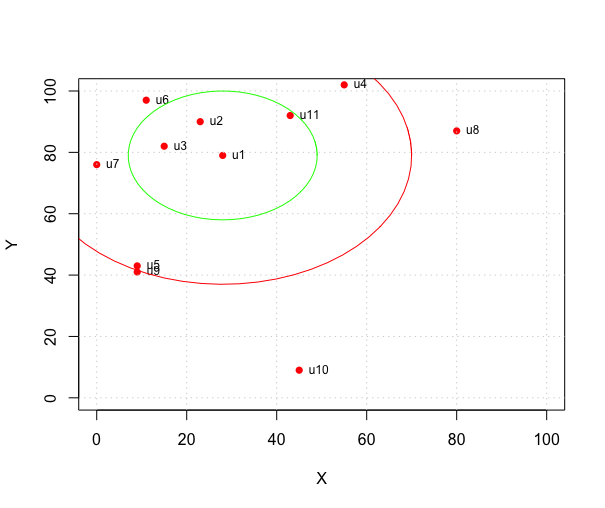
\includegraphics[height=0.6\textwidth]{images/user_coordinates.png}
				\caption{The given user coordinates represented in a Cartesian coordinate system with the radius anonymity region of 42 units (red) and 21 units (green) radius around $u_1$.}
				\label{user_coordinates}
			\end{center}
		\end{figure}
		
		The k-anonymity for each point and radius can be calculated as follows. For each user's coordinate $u_1, u_2...u_n$ we have to check whether they are located inside the circle drawn around $u_1$ with the given radius. If the following inequality, which is derived from the equality of circles, holds
		\begin{equation}
			r <= \sqrt{(x - u)^2 + (y - v)^2}
		\end{equation}
		we can conclude that the investigated point is in the given radius. The number of such points then gives the $k$ value for the anonymity region at all times.
		
		The algorithm below can be used to calculate the k-anonymity values for a set of points (users) with defined central point (user) and radius values. The value of the $counter$ variable will be returned, which indicates the $k$-value of the zone.
		
		\begin{algorithm}
			\caption{K-anonimity}\label{k-anonimity}
				\begin{algorithmic}[1]
					\Procedure{K-anonimity$(points[n], middle\_point, circle\_radius)$}{}
						\State $\textit{counter} \gets \text{0}$
						\For{p in points} 
							\If {\textit{p} in \textit{circle(middle\_point, radius)}}
								\State $counter++$.
							\EndIf
						\EndFor
						\State \Return $counter$
						
					\EndProcedure
			\end{algorithmic}
		\end{algorithm}
		
		An implementation of this algorithm in R language was developed for this task. The corresponding R script file can be found as an attachment to this document. 
	\subsection{Pseudonyms}
	To clarify the given problem, the following observations are made. Each device is expected to have a matching pseudonym, that is
	\begin{itemize}
		\item unique to the device,
		\item does not change over time,
		\item does not change as the software configuration of the device changes (in other words remains the same after performing operating system upgrades or factory reset)
		\item can be retrieved/calculated without internet connection,
		\item hides information concerning the model, manufacturer and software configuration of the device,
		\item hides information about the user of the device.
	\end{itemize}
	
	The above requirements suggest the utilization of hardware parameters for creating such pseudonyms. Accordingly, to guarantee the above requirements, we have to define a device-wide scope and FDR-persistent method for the pseudonyms. Furthermore, the last two items indicate that the pseudonym should not contain any information concerning the device as human-readable, plain text. This indicates some kind of encryption of the previously generated identifier. 
	
	Ensuring the first set of requirements, multiple pieces of information concerning the hardware configuration of the device can be combined as a string. Naturally, the operating system may not have access to all of this information, but this may include:
	\begin{itemize}
		\item the manufacturer of the device (e.g. Samsung, LG, Huawei, etc.),
		\item the model of the device	(e.g. Galaxy S7, Nexus 5s, P9, etc.),
		\item the IMEI (International Mobile Station Equipment Identity) of the device,
		\item the UUID (Universally Unique Identifier) of the device,
		\item the year of manufacturing,
		\item the MAC (Media Access Control) address of the WiFi and/or Bluetooth adapter(s).
	\end{itemize}
	
	To have the best possible outcome, the biggest subset of the available information should be combined universally among the devices. To fulfill the second set of requirements, this information should be encoded. In order to do so, an appropriate encryption algorithm should be selected. For convenience, it would make sense to select a method, that generates a fixed-length string as output. For instance, MD5 generates a 128-bit, SHA-1 generates a 160-bit hash value for every input. Applying one of these or similar encryption methods on the data above hides the human-readable information about the devices. 
	
\section{Energy-efficiency}
	\subsection{Duty cycle}
	Solving the first task requires the following equations: 
	\begin{eqnarray} 
		\Delta t &=& \frac{min(E_{Position}, E_{Trajectory}) - e_{model}}{V_{estimate}} \\
		D &=& \frac{T}{P}
	\end{eqnarray}
	
	Deriving from the description of the task we can see that $v = 3.5 \frac{m}{s}$, $E_{Position} = 50 \, m$, $e = 0 m$. Accordingly, the cycle of refreshing the GPS location of the device is
	
	\begin{eqnarray*}
		\Delta t = \frac{50 m}{3.5 \frac{m}{s}} = \doubleunderline{14.285 \, s}
	\end{eqnarray*}
	
	If the tracking is performed for $P = 10 min = 600 \, s$, and reading the GPS coordinates takes $r = 70 ms = 0,07 \, s$, the GPS location will be refreshed
	
	\begin{eqnarray*}
		n = \floor{\frac{P}{n + r}} = \floor{\frac{600 \, s}{14,285 + 0,7}} = 41
	\end{eqnarray*}
	
	times during the given lifecycle. This yields, that the total active time $T = 41 * 0.07 = 2,87 \, s$. Utilizing the second equation above we can conclude that the duty cycle is
	
	\begin{eqnarray*}
		D = \frac{T}{P} = \frac{2,87}{600} = \doubleunderline{0,47 \%}
	\end{eqnarray*}
	
	If we modify the threshold to $e = 150 \, m$, the calculations modify as follows: 
	
	\begin{eqnarray*}
		\Delta t = \frac{150 \, m}{3.5 \frac{m}{s}} = \doubleunderline{42,85 \, s} \\ \\
		n = \floor{\frac{P}{n + r}} = \floor{\frac{600 \, s}{42,85 + 0,7}} = 13 \\ \\
		T = 13 * 0.07 = 0,91 \, s \\ \\
		D = \frac{T}{P} = \frac{0,91}{600} = \doubleunderline{0,15 \, \%}
	\end{eqnarray*}
	
	\subsection{Android Location API}
	The attached $DutyCycling.java$ file contains some the basics of the implementation for the duty cycling using the Android Location API functions. The attached file is a simple Java class that implements the explained duty cycling mechanism using the Android Location API's functions. The high-level principles of the class are as follows.
	
	The class can be instantiated by passing a $movementSpeed$ and a $treshdold$ value (both are $double$ types). The duty cycling can be started by calling the $start()$ method and stopped by calling the $stop()$ method on the object. The former fires up a timer, which will request the current location coordinates from the service provider, if "sufficient" amount of time has elapsed. The delta time between the refresh-intervals are calculated by the $getDeltaTimeSeconds()$, that relies on the actual value of the $movementSpeed$ class variable (noting that it might change over time). 
	
	As soon as the timer fires up, the algorithm validates if the sufficient time has elapsed. If yes, a request is made to the service provider to query the new coordinates, which is then stored to the $coordinates$ class variable as GIS coordinates in the $refreshCoordinates()$ function. Otherwise, the timer sleeps until the next tick. When the location is refreshed, the $refreshTrackingVariables()$ function is called, which refreshes the $movementSpeed$ and $estimatedError$ variables in order to keep up the duty cycling appropriate to the environmental changes.
	
\pagebreak

\nocite{*}

\bibliographystyle{tktl}
\bibliography{bibliorgaphy}

\lastpage
\appendices
\pagestyle{empty}
\end{document}


